\section{Results and discussion}
\label{sec:res}
%\miniskip
\noindent
\textbf{Performance of non-experts.}
\begin{table}[t!]
\centering
%\resizebox{\textwidth}{!}{
%\begin{tabular}{@{}l@{~~}l@{~~}l@{~~~}l@{~~}l@{~~~}l@{~~}l@{~~~}l@{~~}l@{~~~}l@{~~}l@{~~~}l@{~}l@{}}
\caption{Agreement between experts and non-experts. } 
\begin{tabular}{@{}l@{~~}l@{~~}l@{~~~}l@{~~}l@{~~~}l@{~~}l@{~~~}l@{~~}l@{~~~}l@{~~}l@{~~~}l@{~}l@{}}
\toprule
%& \multicolumn{6}{c}{Species} & \multicolumn{6}{c}{Family} \\
& & \multicolumn{2}{c}{E1} & \multicolumn{2}{c}{E2} & \multicolumn{2}{c}{E3}\\ 
%& \multicolumn{2}{c}{E1} & \multicolumn{2}{c}{E2} & \multicolumn{2}{c}{E3} \\
& & Avg. $\kappa$ & Sdv. & Avg. $\kappa$ & Sdv. & Avg. $\kappa$ & Sdv. \\
%& Avg. $\kappa$ & Sdv. & Avg. $\kappa$ & Sdv. & Avg. $\kappa$ & Sdv.\\
\hline
%U.random & 0.51 & 0.03 & 0.53 & 0.03 & 0.45 & 0.03     & 0.73 & 0.03 & 0.71 & 0.03 & 0.62 & 0.03\\ 
Expr.1 & Species & 0.62 & 0.01 & 0.65 & 0.006 & 0.55 & 0.009 \\  
& Family & 0.83 & 0.008 & 0.81 & 0.01 & 0.72 & 0.009\\
\hline
Expr.2 & Species & 0.65 & 0.009 & 0.50 & 0.008 & 0.45 & 0.009\\
(New)& Family & 0.73 & 0.01 & 0.73 & 0.01 & 0.68 & 0.01\\
\hline
Expr.2 & Species &0.53 & 0.01& 0.68 & 0.01 & 0.64 & 0.02 \\
(Old)& Family & 0.80 & 0.02 & 0.78 & 0.02 & 0.74 & 0.01\\
\bottomrule
\end{tabular}
%}
%(correct labels present).}
\label{tab:agree1}
%\vspace*{-\baselineskip}
\end{table}
%
Table~\ref{tab:agree1} shows the result of label agreement
at both species and family level. 
In terms of Expr.1, 
%
if we compare Table~\ref{tab:agree1} to Table~\ref{tab:expert_agree}, 
%we see that even with a random aggregation, 
we see that the agreement between expert and non-expert labels are rather similar to that among the experts themselves.
%
In terms of Expr.2, we see that the ``new" players (those who only participated in Expr.2)
achieve lower agreements with experts compared to players in Expr.1. 
%
%On the other hand, 
while the performance of ``old'' players is comparable to that of Expr.1.
This to some extent suggests that although the experimental condition has changed, 
the ``training" the players received during Expr.1 has an influence on their performance in Expr.2. 

\begin{table}[t!]
%\vspace*{-\baselineskip}
\centering
\caption{Non-experts' performance evaluated by NDCG.
\dubbelop(\dubbelneer) indicates a significant difference (p-value$<0.01$) tested using Wilcoxon signed-rank test.}
\begin{tabular}{@{}l@{~~}l@{~~}l@{~~}l@{~~}l@{}}
\toprule
 Method & \multicolumn{2}{c}{Species} & \multicolumn{2}{c}{Family}\\
 & NDCG@1 & NDCG@5  & NDCG@1 & NDCG@5\\ 
 \hline
 Expr.1 & 0.84 & 0.88 & 0.93 & 0.94\\
\hline
Expr.2.new & 0.72\dubbelneer  & 0.77\dubbelneer  & 0.86\dubbelneer & 0.94\\
Expr.2.old & 0.88 & 0.86 & 0.91& 0.94\\
\bottomrule
\end{tabular} 
\label{tab:ndcg}
%\vspace*{-\baselineskip}
\end{table}


Further, Table~\ref{tab:ndcg} shows the performance of non-expert labels in terms of NDCG. 
%
In practice, when using the collected labels as training data, often only the label(s) with 
the highest scores are considered as target labels. 
%
Thus it is important that the top ranked labels are correct according
to experts' labels. We list the results of NDCG@1 and 5.  
Unlike the agreement comparison, here we do not 
% directly interpret the results as ``reasonable" or not, 
% as we do not 
have a baseline to compare to.  However, we do see that the scores at least
indicate that for a majority of the images, the non-experts have made correct choices. 
%Since random aggregation only has one chosen label, below NDCG@1, 
%no further gain can be achieved. For majority voting, we see that some other
%relevant candidates are within the top 5 of the ranked list, as the
%scores at NDCG@5 are higher than that at NDCG@1. 
%
%Intuitively, this is a more difficult task for the players, as we deliberately removed
%the target labels of some of the query images, and left in candidates that are similar but not actually relevant. 
%Table~\ref{tab:ndcg2} lists the results in terms of NDCG. 
The new players in Expr.2 have a significant lower performance compared to
Expr.1, while the performance of ``old" users do not show significant difference compared to 
that achieved in Expr.1. 
%both with random aggregation and majority voting. 
%The differences are statistically significant. 
%
%The old players in Expr. 2 perform better than
%those in Expr. 1 when labels are randomly aggregated. 
%There is no significant difference
%between the results of majority voting. It could be that the ``old'' players are well-trained
%when they participated in Expr. 2 % while in Expr. 1, the players have to start from scratch 
%and therefore with random aggregation, their labels are more robust.% with those ``old'' players in Expr. 2.
%
%\todo{A comparison between the new player of experiment 1 and 2 is needed.}
%We see that 
%In general the new players in Expr. 2 perform worse compared to
%Expr. 1. 
We consider two potential explanations: 1)~the set up of Expr.2 makes a more
difficult task for novice players; or 2)~since most of the new players did only one session, the general quality of the labels 
are not as good as that of Expr.1, where many played more than one session. 
To distinguish the two cases, we verify if the results from only the first session of each player in Expr.1 still outperform 
that of Expr.2.
% If so, we could probably trust more that there is a difference between the difficulty of the tasks defined in the two experiments. 
%
In Table~\ref{tab:ndcg3} we see that indeed,  a significant difference exists between the performance
of the first session labels in the two experiments. That is, when target labels are absent
while similar non-target labels are present, novice players are more likely to be confused.
%
This suggests that selecting a good set of candidate labels is important. 
%
\begin{table}[t!]
%\vspace*{-\baselineskip}
\centering
\caption{Comparing the performance in the first sessions under Expr. 1 and 2. 
Only ``new'' players are considered. Wilcoxon signed-rank test is used for significance testing.}
\begin{tabular}{@{}l@{~~}l@{~~}l@{~~}l@{~~}l@{~~}l@{~~}l@{}}
\toprule
Method & \multicolumn{2}{c}{Species} & \multicolumn{2}{c}{Family}\\
& NDCG@1 & NDCG@5  & NDCG@1 & NDCG@5\\ 
% \multirow{3}{*}{U.Random}
%&T1   & 0.72 & 0.67 & 0.84 & 0.82 \\ 
%&T2   & 0.60 & 0.57 & 0.76\dubbelneer & 0.77\dubbelneer\\
\hline
%\multirow{3}{*}{U.MVote}
Expr.1 & 0.84 & 0.88 & 0.93 & 0.94\\
Expr.2 & 0.72\dubbelneer & 0.77\dubbelneer& 0.86\dubbelneer & 0.94\\  
\bottomrule
\end{tabular}
%\vspace*{-\baselineskip}
\label{tab:ndcg3}
\end{table}

\noindent
\textbf{Do non-experts learn?}
%\label{subsec:res_learn}
%Figure~\ref{fig:learn} illustrates players' performance over time, evaluated as described in Section~\ref{sec:eval}.
%As discussed in Section~\ref{subsec:nonexpt_exp}, 
%The box plots are constructed over all players and all images labeled in each experiment. 
%
\begin{table}[t!]
%\vspace*{-\baselineskip}
\centering
\caption{The impact of learning over time. 
%We use Wilcoxon rank-sum test~\cite{Wilcoxon45} for 
%significance testing. 
%\dubbelop indicates a significant difference with p-value$<$0.01. 
Wilcoxon rank-sum test is used for significance testing.
All comparisons are between the first label and the $nth$ label.}
\resizebox{\columnwidth}{!}{
\begin{tabular} {@{}l@{~~}l@{~~}l@{~~}l@{~~}l@{~~} | @{~~}l@{~~}l@{~~}l@{~~}l@{~~}l@{~~}l@{}}
\toprule
& \multicolumn{4}{c}{Memorizing} & \multicolumn{5}{c}{Generalization}\\
\hline
Labels & 1 & 2 & 3 & 4  & 1 & 5 & 10 & 15 & 20 & 25\\
\hline
Expr.1 & 0.30 & 0.38\dubbelop & 0.46\dubbelop & 0.51\dubbelop & 0.42 & 0.51\dubbelop & 0.59\dubbelop & 0.63\dubbelop & 0.67\dubbelop & 0.70\dubbelop\\
Expr.2.new & 0.30 & 0.40\dubbelop & 0.44\dubbelop & 0.52\dubbelop & 0.37 & 0.58\dubbelop  & 0.62\dubbelop  & - & - & -\\
\bottomrule
\end{tabular}
}
\label{tab:effect}
%\vspace*{-\baselineskip}
\end{table}
%
%We see from Figure~\ref{fig:learn} that the scores of the first labels are in all cases relatively 
%low, with a relatively large variance, compared to the following up labels\footnote{The results in Tabel~\ref{tab:effect}
%should not be confused with performance of aggregated labels, e.g., Tables~\ref{tab:ndcg}--\ref{tab:ndcg3}.
%Results here include cases when ``others'' are correctly chosen but target labels are not present, while the results
%of aggregated labels do not include these cases.}. 
%In the cases of memorization, initially, the difference between the scores of the first and second labels 
%seem to be more obvious compared to that of later labels. In the case of generalization, there seems to have 
%a trend of continuous improvement over time.  
%
Table~\ref{tab:effect} shows the comparison of the averaged scores achieved 
at the first label for an image to that of  the nth labels.
%
These numbers %in Table~\ref{tab:effect} 
confirms that there is a significant difference 
between the scores achieved with the first label and those achieved over time, in both 
experiments non-experts can learn and improve their labels over time. 
They do not only learn to provide more accurate labels for images that they have seen 
before, but also for similar images, i.e., different images that contain species that they have seen before. 


%=============OLD==============
\if 0
\section{Results and discussion}
\label{sec:res}
%We now proceed to the experimental results.
% \subsection{Can non-expert identify the correct labels?}
%
%\miniskip
\begin{table*}[t!]
\centering
%\resizebox{\textwidth}{!}{
\begin{tabular}{@{}l@{~~}l@{~~}l@{~~~}l@{~~}l@{~~~}l@{~~}l@{~~~}l@{~~}l@{~~~}l@{~~}l@{~~~}l@{~}l@{}}
\hline
& \multicolumn{6}{c}{Species} & \multicolumn{6}{c}{Family} \\
& \multicolumn{2}{c}{E1} & \multicolumn{2}{c}{E2} & \multicolumn{2}{c}{E3} & \multicolumn{2}{c}{E1} & \multicolumn{2}{c}{E2} & \multicolumn{2}{c}{E3} \\
& Avg. $\kappa$ & Sdv. & Avg. $\kappa$ & Sdv. & Avg. $\kappa$ & Sdv. & Avg. $\kappa$ & Sdv. & Avg. $\kappa$ & Sdv. & Avg. $\kappa$ & Sdv.\\
\hline
U.random & 0.51 & 0.03 & 0.53 & 0.03 & 0.45 & 0.03     & 0.73 & 0.03 & 0.71 & 0.03 & 0.62 & 0.03\\ 
U.MVote & 0.62 & 0.01 & 0.65 & 0.006 & 0.55 & 0.009   & 0.83 & 0.008 & 0.81 & 0.01 & 0.72 & 0.009\\
\hline
\end{tabular}
%}
\caption{Agreement (Cohen's kappa) between experts and non-experts  (correct labels present).}
\label{tab:agree1}
%\vspace*{-\baselineskip}
\end{table*}

\subsection{Performance when target labels are present}

Table~\ref{tab:agree1} shows the result of label agreement
at both species level and family level. 
If we compare Table~\ref{tab:agree1} to Table~\ref{tab:expert_agree}, we see that 
even with a random aggregation, the agreement between expert and non-expert 
labels are rather similar to that among the experts themselves.
Recall that the $\kappa$ values of experts agreement ranges from 0.48 to 0.67 at
the species level and from 0.75 to 0.85 at the family level. 
%
The result of majority voting has a stronger agreement with the experts compared
to the random aggregation results. This indicates that the crowd can, to some extent, correct
errors made by individuals. 

Further, Table~\ref{tab:ndcg} shows the performance of non-expert labels in terms of NDCG. 
%
In practice, when using the collected labels as training data, often only the label(s) with 
the highest scores will be considered as target labels. 
%
Therefore it is important that the very top ranked labels are the correct ones according
to experts' labels, we list the results of NDCG@1 and 5.  
Unlike the agreement comparison, here we do not 
% directly interpret the results as ``reasonable" or not, 
% as we do not 
have a baseline to compare to.  However, we do see that the scores at least
indicate that for a majority of the images, the non-experts have made correct choices. 
Since random aggregation only has one chosen label, below NDCG@1, 
no further gain can be achieved. For majority voting, we see that some other
relevant candidates are within the top 5 of the ranked list, as the
scores at NDCG@5 are higher than that at NDCG@1. 
%
\begin{table}[h!]
%\vspace*{-\baselineskip}
\centering
\begin{tabular}{@{}l@{~~}l@{~~}l@{~~}l@{~~}l@{}}
\hline
 Method & \multicolumn{2}{c}{Species} & \multicolumn{2}{c}{Family}\\
 & NDCG@1 & NDCG@5  & NDCG@1 & NDCG@5\\ 
 \hline
 U.random & 0.71 & 0.67 & 0.85 & 0.82\\
 U.MVote & 0.84 & 0.88 & 0.93 & 0.94\\
\hline
\end{tabular}
\caption{Non-experts' performance evaluated by NDCG (correct labels present).}
\label{tab:ndcg}
%\vspace*{-\baselineskip}
\end{table}
%
%In consistence with the results shown in the previous section, the MAP aggregation
%method achieves better results compared to that of BC. 
%In particular, the difference is more obvious at the top of the ranked list, e.g., in terms of NDCG@1.  
%This suggests that MAP is a more effective aggregation method than BC for our task, where the correctness
%of the very top ranked labels is important. 

In summary, when present among the candidates, in most cases the target labels 
can be identified by the players.
%
In particular, the agreement achieved between the non-experts and the experts
are comparable to that achieved among the experts themselves. 

% \miniskip
\subsection{Performance when some target labels are absent}
%\todo{Random T2 player performance are not as good as T1, but majority voting can help.}
%\todo{Old players, although we only have 4 with 9 sessions, they show that they are not performing worse than 
%in T1, may because they are well-trained. this suggest: 1) if players are well-trained, they are more robust against
%system performance, e.g., if we use an imperfect candidate selection algorithm; 2) if players are new and the system
%is not perfect, the crowd can still provide some help.}

%Now let us proceed to the result of the second experiment. 
Intuitively, this is a more difficult task for the players, as we deliberately removed
the target labels of some of the query images, and left in candidates that are similar but not actually relevant. 

%
\begin{table*}[t!]
%\vspace*{-\baselineskip}
\centering
%\resizebox{\textwidth}{!}{
\begin{tabular}{@{~~}l@{~~}l@{~~}l@{~~}l@{~~~}l@{~~}l@{~~~}l@{~~}l@{~~~}l@{~~}l@{~~~}l@{~~}l@{~~~}l@{~}l@{}}
\hline
User&Method& \multicolumn{6}{c}{Species} & \multicolumn{6}{c}{Family} \\
& & \multicolumn{2}{c}{E1} & \multicolumn{2}{c}{E2} & \multicolumn{2}{c}{E3} & \multicolumn{2}{c}{E1} & \multicolumn{2}{c}{E2} & \multicolumn{2}{c}{E3} \\
& & Avg. $\kappa$ & Sdv. & Avg. $\kappa$ & Sdv. & Avg. $\kappa$ & Sdv. & Avg. $\kappa$ & Sdv. & Avg. $\kappa$ & Sdv. & Avg. $\kappa$ & Sdv.\\
\hline
\multirow{2}{*}{New}
& U.random & 0.47 & 0.03 & 0.37 & 0.03 & 0.36 & 0.03     & 0.60 & 0.03 & 0.59 & 0.04 & 0.58 & 0.04\\ 
& U.MVote & 0.65 & 0.009 & 0.50 & 0.008 & 0.45 & 0.009  & 0.73 & 0.01 & 0.73 & 0.01 & 0.68 & 0.01\\
\hline
\multirow{2}{*}{Old}
& U.random & 0.52 & 0.02 & 0.67 & 0.02 & 0.62 & 0.02 & 0.79 & 0.02 & 0.77 & 0.02 & 0.71 & 0.02\\
& U.MVote   & 0.53 & 0.01& 0.68 & 0.01 & 0.64 & 0.02 & 0.80 & 0.02 & 0.78 & 0.02 & 0.74 & 0.01\\
\hline
\end{tabular}
%}
\caption{Agreement (Cohen's kappa) between experts and non-experts (some labels missing)}
\label{tab:agree2}
%\vspace*{-\baselineskip}
\end{table*}
%
Table~\ref{tab:agree2} shows the agreement between the non-experts and the experts.
%As mentioned in Section~\ref{subsec:data_nonexp}, we treat the ``new'' and ``old'' players separately.
The ``new" players are those who only participated in Expr. 2, 
while ``old" players participated in both experiments.
We see that for new players, the randomly aggregated labels have a much lower agreement with the experts
compared to those in Table~\ref{tab:agree1}.
However, the results after majority voting are much better. 
%
This suggests that % for new players  the individual performance is low, but 
the crowd can help to correct some of the errors made by new individual players. 
%\todo{effect bigger than in exp 1?}
%
On the other hand, ``old'' players perform comparable to the results in Table~\ref{tab:agree1}.
Since we only have 4 old players, random aggregation is not very different from majority voting.
%
\begin{table}[ht!]
%\vspace*{-\baselineskip}
\centering
\begin{tabular}{@{}l@{~~}l@{~~}l@{~~}l@{~~}l@{~~}l@{~~}l@{}}
\hline
Method &Users & \multicolumn{2}{c}{Species} & \multicolumn{2}{c}{Family}\\
& & NDCG@1 & NDCG@5  & NDCG@1 & NDCG@5\\ 
 \hline
 \multirow{3}{*}{U.Random}
&T1        & 0.71 & 0.67 & 0.85 & 0.82\\
&T2.new & 0.52\dubbelneer & 0.50\dubbelneer & 0.66\dubbelneer & 0.68\dubbelneer\\
&T2.old   & 0.86\dubbelop & 0.81\dubbelop & 0.91\dubbelop & 0.91\dubbelop\\
\hline
\multirow{3}{*}{U.MVote}
&T1 & 0.84 & 0.88 & 0.93 & 0.94\\
&T2.new & 0.72\dubbelneer  & 0.77\dubbelneer  & 0.86\dubbelneer & 0.94\\
&T2.old & 0.88 & 0.86 & 0.91& 0.94\\
\hline
\end{tabular}
\caption{Comparing the performance of players under Expr. 1 (T1) and 2 (T2) (``new" and ``old" players).
%.new refers to new players; .old refers to old players.
%of players under the settings of experiment 2 to that 
%under the settings of experiment1, in terms of NDCG. T1 refers to experiment 1; T2.new refers
%to experiment 2 with new players; and T2.old refers experiment 2 with old players from experiment 1. 
\dubbelop(\dubbelneer) indicates a significant difference tested using Wilcoxon signed-rank test~\cite{Wilcoxon45}. }
\label{tab:ndcg2}
%\vspace*{-\baselineskip}
\end{table}
%
Table~\ref{tab:ndcg2} lists the results in terms of NDCG. 
The new players in Expr. 2 have a significantly lower performance compared to
Expr. 1, both with random aggregation and majority voting. 
%The differences are statistically significant. 
%
The old players in Expr. 2 perform better than
those in Expr. 1 when labels are randomly aggregated. There is no significant difference
between the results of majority voting. It could be that the ``old'' players are well-trained
when they participated in Expr. 2 % while in Expr. 1, the players have to start from scratch 
and therefore with random aggregation, their labels are more robust.% with those ``old'' players in Expr. 2.
%
%\todo{A comparison between the new player of experiment 1 and 2 is needed.}
%We see that 
In general the new players in Expr. 2 perform worse compared to
Expr. 1. 
We consider two potential explanations: 1)~the set up of Expr. 2 makes a more
difficult task for novice players; or 2)~since most of the new players did only one session, the general quality of the labels 
are not as good as that of Expr. 1, where many played more than one session. 
To distinguish the two cases, we verify if the results from only the first session of each player in Expr. 1 still outperform 
that of Expr. 2.
% If so, we could probably trust more that there is a difference between the difficulty of the tasks defined in the two experiments. 
%
In Table~\ref{tab:ndcg3} we see that indeed, there is a significant difference between the performance
of the first session labels in the two experiments. That suggests that when target labels are absent
while similar non-target labels are present, the novice players are more likely to be confused.
%
This confirms our intuition that selecting a good set of candidate labels is very important. 
%
\begin{table}[h!]
%\vspace*{-\baselineskip}
\centering
\begin{tabular}{@{}l@{~~}l@{~~}l@{~~}l@{~~}l@{~~}l@{~~}l@{}}
\hline
Method &Users & \multicolumn{2}{c}{Species} & \multicolumn{2}{c}{Family}\\
& & NDCG@1 & NDCG@5  & NDCG@1 & NDCG@5\\ 
 \hline
 \multirow{3}{*}{U.Random}
&T1   & 0.72 & 0.67 & 0.84 & 0.82 \\ 
&T2   & 0.60 & 0.57 & 0.76\dubbelneer & 0.77\dubbelneer\\
\hline
\multirow{3}{*}{U.MVote}
&T1 & 0.84 & 0.88 & 0.93 & 0.94\\
&T2 & 0.72\dubbelneer & 0.77\dubbelneer& 0.86\dubbelneer & 0.94\\  
\hline
\end{tabular}
\label{tab:ndcg3}
\caption{Comparing the performance in the first sessions under Expr. 1 (T1) and 2 (T2). 
In T2, only ``new'' players are considered. Wilcoxon signed-rank test is used for significance testing.}
%\vspace*{-\baselineskip}
\end{table}
%



%Table~\ref{tab:species_agree} and Table~\ref{tab:family_agree} show the result of annotation agreement
%at both species level and family level, respectively.
%E1, E2, and E3 represent the three marine biologists, and E* is the aggregated expert annotation.
%U.Vote and U.MAP are the two aggregated non-expert annotations, where U.Vote uses Borda count and U.MAP
%uses maximum a posteriori as aggregation method. 

%We have a number of observations here. 
%First, we see that among the expert annotations, the agreement is rather moderated at the species level.
%As expected, at family level the agreement is relatively strong.  
%This indicates that the annotation task at species level is perhaps difficult even for experts. 

%Second, we see that the agreement between non-experts and experts is influenced by the aggregation method. 
%U.Vote has a generally lower agreement with each of the experts as well as the aggregated expert annotation, compared to that between the expert annotations. 
%However, U.MAP achieves an agreement with the experts that is rather close to the agreement among the experts. 
%In some cases, U.MAP even has a higher agreement with one of the expert annotation compared to other experts.
%For instance at species level, we see that $\kappa(\textit{E1, U.MAP})>\kappa(\textit{E1, E2 or E3})$; and at family level, 
%we see $\kappa(\textit{E1, U.MAP})>\kappa(\textit{E1, E3})$.
%These observations suggest that with a proper aggregation method, the non-expert annotation can achieve an agreement with the expert annotations that is comparable to that between the experts. 


%\begin{table}[h]
%\centering
%\begin{tabular}{@{}l@{~~}l@{~~}l@{~~}l@{~~}l@{}}
%\hline
% Method & \multicolumn{2}{c}{Species} & \multicolumn{2}{c}{Family}\\
% & NDCG@1 & NDCG@5  & NDCG@1 & NDCG@5\\ 
% \hline
% U.random & 0.71 & 0.67 & 0.85 & 0.82\\
% %U.random & 0.71 & 0.68 & 0.67 & 0.85 & 0.82 & 0.82\\
% %U.Vote & 0.52 & 0.68 & 0.71 & 0.66 & 0.79 & 0.82\\
% %U.MAP & 0.79 & 0.81 & 0.82 & 0.91 & 0.91 & 0.92\\
% U.MVote & 0.84 & 0.88 & 0.93 & 0.94\\
% %U.MVote & 0.84 & 0.87 & 0.88 & 0.93 &  0.94 & 0.94\\
% %U.Zscore & 0.78 & 0.79 & 0.81 &0.91 & 0.90 &0.91\\
%\hline
%\end{tabular}
%\caption{Non-experts' performance evaluated by NDCG.}
%\label{tab:ndcg}
%\end{table}


%Table~\ref{tab:pearson} verifies our hypothesis described in Section~\ref{subsec:eval_ndcg}. 
%We see that the entropy of the labels assigned to an image has a significant negative correlation with
%the its performance in terms of NDCG, with respect to both aggregation methods.  
%That is, if many diverse labels are assigned to an image, the image is likely to be a difficult one and
%and the annotation is likely to have low performance.  


%\begin{table}[h]
%\centering
%\begin{tabular}{@{}l@{~~}l@{~~}l@{~~}l@{~~}l@{~~}l@{~~}l@{~~}l@{}}
%\hline
%Label type& Method & \multicolumn{3}{c}{Species} & \multicolumn{3}{c}{Family}\\
%& & NDCG@1 & NDCG@3 & NDCG@5  & NDCG@1 & NDCG@3 & NDCG@5\\ 
% \hline
% \multirow{2}{*}{Non-experts}
%& U.Vote & -0.42\dubbelop & -0.62\dubbelop & -0.63\dubbelop & -0.33\dubbelop & -0.43\dubbelop & -0.40\dubbelop \\
%& U.MAP &  -0.56\dubbelop & -0.58\dubbelop & -0.59\dubbelop & -0.37\dubbelop & -0.38\dubbelop & -0.37\dubbelop\\
%& U.MVote & -0.39\dubbelop & -0.49\dubbelop & -0.51\dubbelop & -0.30\dubbelop & -0.22\dubbelop & -0.18\enkelop\\
%& U.Random & -0.77\dubbelop & -0.74\dubbelop & -0.78\dubbelop & -0.58 \dubbelop& -0.55\dubbelop & -0.55\dubbelop\\ 
%& U.Zscore & -0.59\dubbelop & -0.61\dubbelop & -0.61\dubbelop & -0.34\dubbelop & -0.37\dubbelop & -0.36\dubbelop\\
%\hline
%%
% \multirow{2}{*}{Experts}
%& U.Vote & -0.02 & -0.07 & -0.10 & -0.02 & -0.04 & -0.05 \\
%& U.MAP &  -0.11 & -0.20\dubbelop & -0.26\dubbelop & -0.02 & -0.07 & -0.07\\
%& U.Mvote & -0.19\dubbelop & -0.41\dubbelop & -0.44\dubbelop & -0.15\enkelop & -0.13 & -0.13\\  
%& U.Random & -0.24\dubbelop & -0.44\dubbelop & -0.50\dubbelop & -0.12 & -0.22\dubbelop & -0.22\dubbelop\\
%& U.Zscore & -0.12 & -0.18\enkelop & -0.24\dubbelop & -0.02 & -0.076 & -0.08\\
%\hline
%%
%\end{tabular}
%\caption{Pearson correlation ($\rho$) between player performance in terms of NDCG and label entropy. 
%\dubbelop (\enkelop) indicates a significant correlation with p-value $<$ 0.01 (0.05). }
%\label{tab:pearson}
%\end{table}

%\miniskip
\subsection{Do non-experts learn?}
%\label{subsec:res_learn}
Figure~\ref{fig:learn} illustrates players' performance over time, evaluated as described in Section~\ref{sec:eval}.
%As discussed in Section~\ref{subsec:nonexpt_exp}, 
The box plots are constructed over all players and all images labeled in each experiment. 
Table~\ref{tab:effect} shows the comparison of the averaged scores achieved 
at the first label for an image to that of  the nth labels. %(See Eq.~\ref{eq:score_t}). 
%The nth label refers to the nth time a player sees the same image, or a different image from the same
%species in case of generalization. 
%
%Notice that not all image (or category in the case of generalization) have been repeatedly shown 
%to the players for the same number of times. For example, in Experiment 1 
%there are 785 images that have been shown at least once\footnote{Note that this number is not 
%the unique number of images, as we aggregate over all annotators.}, while only 3 have been shown 
%6 times. In order to have a reliable result for statistical comparison, we exclude the images that 
%only appeared once and only include the label orders (i.e., the nth time a label is given to an image 
%by an annotator) that involve more than 30 images/categories. 
%In the case of memorization, we consider up till the 4th label, and in the case of generalization, 
%we consider up till the 25th label for Experiment 1 and 10th label for Experiment 2.
%
%\todo{I'm totally confused here.  Should this not be moved to section 5?}
%
\begin{table}[h!]
%\vspace*{-\baselineskip}
\centering
\resizebox{\columnwidth}{!}{
\begin{tabular} {@{}l@{~~}l@{~~}l@{~~}l@{~~}l@{~~} | @{~~}l@{~~}l@{~~}l@{~~}l@{~~}l@{~~}l@{}}
\hline
& \multicolumn{4}{c}{Memorizing} & \multicolumn{5}{c}{Generalization}\\
\hline
Labels & 1 & 2 & 3 & 4  & 1 & 5 & 10 & 15 & 20 & 25\\
\hline
T1 & 0.30 & 0.38\dubbelop & 0.46\dubbelop & 0.51\dubbelop & 0.42 & 0.51\dubbelop & 0.59\dubbelop & 0.63\dubbelop & 0.67\dubbelop & 0.70\dubbelop\\
T2.new & 0.30 & 0.40\dubbelop & 0.44\dubbelop & 0.52\dubbelop & 0.37 & 0.58\dubbelop  & 0.62\dubbelop  & - & - & -\\
\hline
\end{tabular}
}
\caption{The impact of learning over time. 
%We use Wilcoxon rank-sum test~\cite{Wilcoxon45} for 
%significance testing. 
%\dubbelop indicates a significant difference with p-value$<$0.01. 
Wilcoxon rank-sum test is used for significance testing.
All comparisons are between the first label and the $nth$ label.}
\label{tab:effect}
%\vspace*{-\baselineskip}
\end{table}
%
We see from Figure~\ref{fig:learn} that the scores of the first labels are in all cases relatively 
low, with a relatively large variance, compared to the following up labels\footnote{The results in Tabel~\ref{tab:effect}
should not be confused with performance of aggregated labels, e.g., Tables~\ref{tab:ndcg}--\ref{tab:ndcg3}.
Results here include cases when ``others'' are correctly chosen but target labels are not present, while the results
of aggregated labels do not include these cases.}. 
In the cases of memorization, initially, the difference between the scores of the first and second labels 
seem to be more obvious compared to that of later labels. In the case of generalization, there seems to have 
a trend of continuous improvement over time.  
%
\begin{figure*}[t!]
%\vspace*{-\baselineskip}
\subfigure[]{
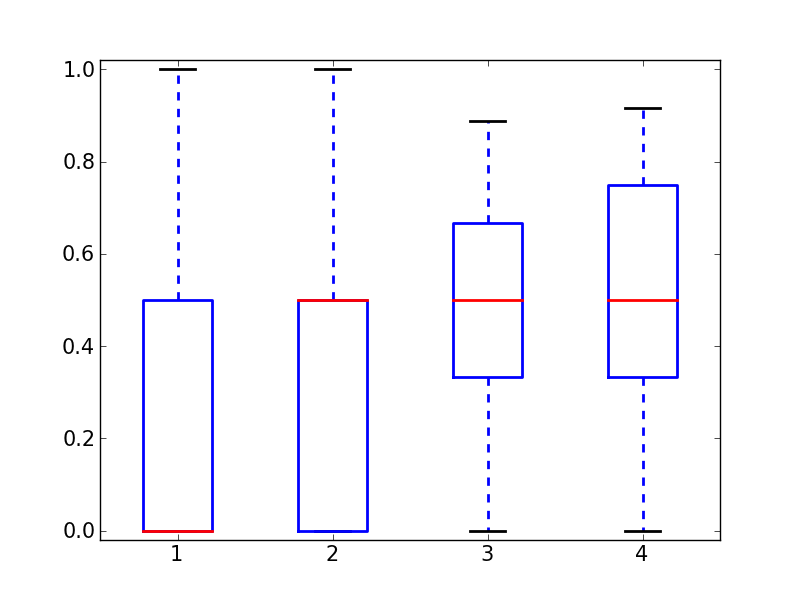
\includegraphics[width=0.45\textwidth, height=0.25\textwidth]{box_repimg.png}
%\miniskip
\label{fig:memo_t1}
}
\subfigure[]{
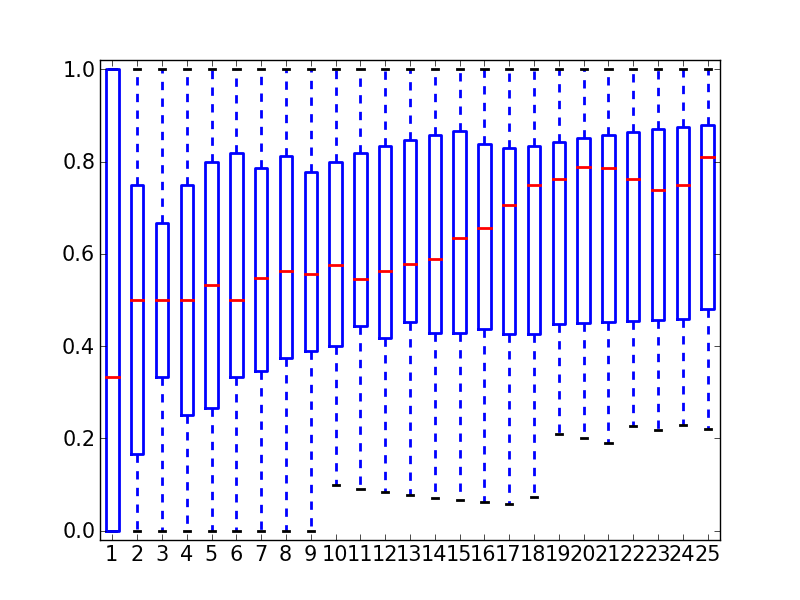
\includegraphics[width=0.45\textwidth, height=0.25\textwidth]{box_speciesimg.png}
%\miniskip
\label{fig:gene_t1}
}
\\
\subfigure[]{
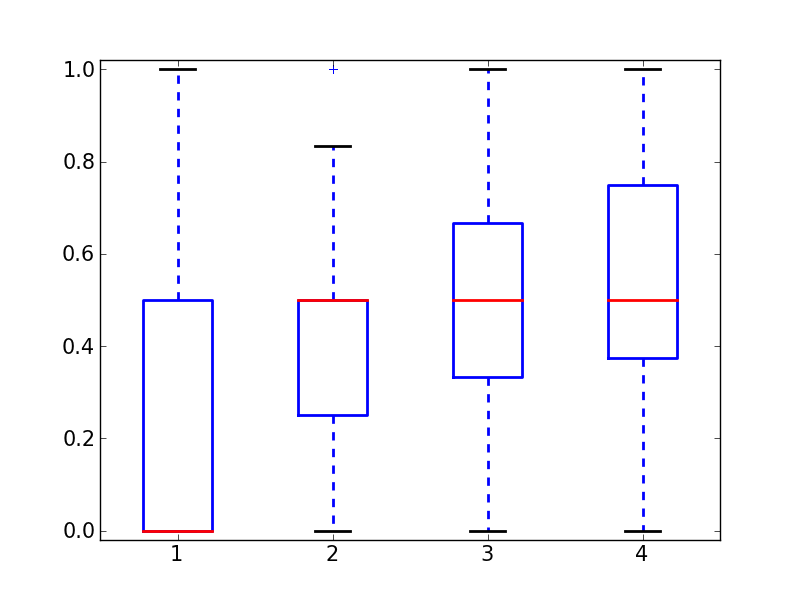
\includegraphics[width=0.45\textwidth, height=0.25\textwidth]{memo_t2.png}
%\miniskip
\label{fig:memo_t2}
}
\subfigure[]{
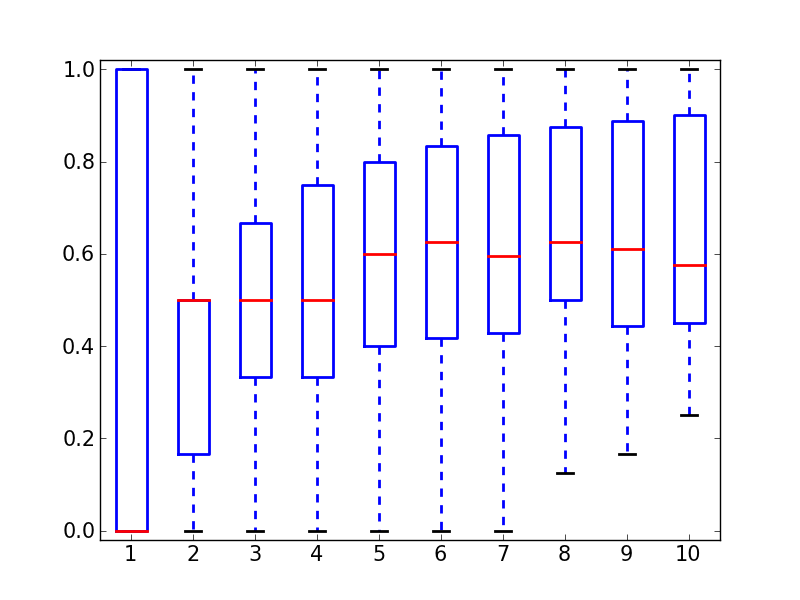
\includegraphics[width=0.45\textwidth, height=0.25\textwidth]{gene_t2.png}
%\miniskip
\label{fig:gene_t2}
}
\caption{The learning behavior of non-experts: memorizing (left) 
and generalization (right). Figures~\ref{fig:memo_t1} and~\ref{fig:gene_t1} are result of Experiment 1;
Figure~\ref{fig:memo_t2} and~\ref{fig:gene_t2} are result of Experiment 2.}
\label{fig:learn}
%\vspace*{-\baselineskip}
\end{figure*}
%
The numbers in Table~\ref{tab:effect} confirms that there is a significant difference 
between the scores achieved with the first label and those achieved over time, in both 
experiments non-experts can learn and improve their labels over time. 
They do not only learn to provide more accurate labels for images that they have seen 
before, but also for similar images, i.e., different images that contain species that they have seen before. 


\fi

%\todo{Maybe to the conclusion: While we can not conclusively say that the annotators learn from the 
%system feedbacks, as many other factors can contribute to their improvement, e.g., 
%they may get used to the quality of the images over time, we do believe that the system feedback is 
%a major reason that the annotators are able to improve their performance. Some annotators 
%explicitly explained how they approach to achieve higher points as well as their experience of 
%memorizing the options that give them highest points. In order to have a better understanding of 
%how annotators learn during the annotation process and what makes the learning most effective, 
%more controlled experiments are needed. This is however out of the scope of this paper.} 





%\begin{table}
%\centering
%\begin{tabular}{@{}l@{~~}l@{~}l@{~~~}l@{~}l@{~~~}l@{~}l@{~~~}l@{~}l@{}}
%\hline
%& \multicolumn{2}{c}{E1} & \multicolumn{2}{c}{E2} & \multicolumn{2}{c}{E3} & \multicolumn{2}{c}{E*} \\
%& Avg. $\kappa$ & Sdv. & Avg. $\kappa$ & Sdv. & Avg. $\kappa$ & Sdv. & Avg. $\kappa$ & Sdv. \\
%\hline
%E1 & - & - & - & - & - & - & 0.59 & 0.01 \\
%E2 & 0.55 & 0.008 &  - & - & - & - & 0.55 & 0.001\\
%E3 & 0.48 & 0.008 & 0.67 & 0.006 & - & -  & 0.52 & 0.07 \\
%U.random & 0.51 & 0.03 & 0.53 & 0.03 & 0.45 & 0.03 & - & - \\ 
%U.Vote  & 0.35 & 0.009 & 0.34 & 0.004 & 0.31 & 0.006 & 0.30 & 0.01\\
%U.MAP & 0.58 & 0.01 & 0.55 & 0.001 & 0.49 & 0.006 & 0.46 & 0.03  \\ 
%U.MVote & 0.62 & 0.01 & 0.65 & 0.006 & 0.55 & 0.009 \\
%U.Zscore & 0.55 & 0.009 & 0.57 & 0.005 & 0.49 & 0.008 \\
%\hline
%\end{tabular}
%\caption{Cohen's kappa for measuring annotation agreement at species level.}
%\label{tab:species_agree}
%\end{table}
%
%\begin{table}
%\centering
%\begin{tabular}{@{}l@{~~}l@{~}l@{~~~}l@{~}l@{~~~}l@{~}l@{~~~}l@{~}l@{}}
%\hline
%& \multicolumn{2}{c}{E1} & \multicolumn{2}{c}{E2} & \multicolumn{2}{c}{E3} & \multicolumn{2}{c}{E*} \\
%& Avg. $\kappa$ & Sdv. & Avg. $\kappa$ & Sdv. & Avg. $\kappa$ & Sdv. & Avg. $\kappa$ & Sdv. \\
%\hline
%E1 & - & - & - & - & - & - & 0.71 & 0.01 \\
%E2 & 0.85 & 0.004 &  - & - & - & - & 0.66 & 0.01\\
%E3 & 0.75 & 0 & 0.76 & 0.0001 & - & -  & 0.83 & 0.01 \\
%U.random & 0.73 & 0.03 & 0.71 & 0.03 & 0.62 & 0.03 & - & -\\
%U.Vote  & 0.53 & 0.01 & 0.49 & 0.12 & 0.47 & 0.009 & 0.41 & 0.01\\
%U.MAP & 0.83 & 0.004 & 0.78 & 0 & 0.70 & 0 & 0.69 & 0.01  \\ 
%U.MVote & 0.83 & 0.008 & 0.81 & 0.01 & 0.72 & 0.009\\
%U.Zscore& 0.82 & 0.005 & 0.78 & 0.003 & 0.69 & 0.0001\\
%\hline
%\end{tabular}
%\caption{Cohen's kappa for measuring annotation agreement at family level. }
%\label{tab:family_agree}
%\end{table}


%\begin{itemize}
%\item Agreement between 3 experts: Fliess' kappa for multi-rater agreement.
%\item At species level, sometimes experts assign multiple labels to a single image, including cases such as
%they are not sure between species A and B as well as cases where they assign labels at family level.
%To cope with this situation, we randomly choose one of the multiple labels a biologist assigned to an image. 
%We repeat this process for 1000 times and report the average as well as standard deviation of 
%Fleiss' kappa calculated in this way. The agreement calculated this way is conservative.
%\item We look at both species level and family level. 
%\item To measure agreement between expert and players, we aggregate player judgement to a single
%rating of the candidate categories. Then we replace one of the 3 experts using this aggregated
%player rating and calculate the agreement.
%\item We take the candidates with the highest rating scores as the labels assigned by the players. 
%\end{itemize}

%\begin{table}
%\centering
%\begin{tabular}{@{}l@{~~}l@{~~}l@{~~}l@{~~}l@{}}
%\hline
%Agreement & \multicolumn{2}{c}{Species} & \multicolumn{2}{c}{Family}\\
%& Avg. $\kappa$& Stdv. & Avg. $\kappa$ & Stdv.\\ 
%\hline
%Expt. vs. Expt & 0.56 & 0.005 & 0.78 & 0.001\\
%\hline
%U.MAP vs. Expt$^{1,2}$& 0.57 & 0.002 & 0.74 & 0\\
%U.MAP vs. Expt$^{1,3}$& 0.51 & 0.005 & 0.76 & 0.001\\
%U.MAP vs. Expt$^{2,3}$& 0.56 & 0.004 & 0.82 & 0.002\\
%\hline
%U.Vote vs. Expt$^{1,2}$& 0.43 & 0.003 & 0.56 & 0.006\\
%U.Vote vs. Expt$^{1,3}$& 0.37 & 0.004 & 0.58 & 0.006\\
%U.Vote vs. Expt$^{2,3}$& 0.41 & 0.004 & 0.61 & 0.008\\
%\hline
%\end{tabular}
%\caption{Fliess' kappa for agreement, 1000 runs}
%\end{table}
